\section{Valid Elimination at the Candidate level}

    For addressing the validity of eliminations under our memory model, we separately address first Read elimination, followed by Write elimination, both at the candidate level. 
    At the Candidate level, eliminating an event would imply removal of certain ordering relations at the Candidate Execution level. 
    Given an event $e$ belonging to a Candidate $C$, the candidate $C'$ after eliminating event $e$ from it would imply no relations of the form 
    \begin{align*}
        \reln{k}{ao}{e} \\  
        \reln{e}{ao}{k}.
    \end{align*}
    and no relations of the form
    \begin{align*}
        \reln{k}{hb}{e} \\
        \reln{e}{hb}{k}.
    \end{align*}
    exist in any Candidate Execution of $C'$.
    
    %Read Elimination 
    \subsection{Elimination of Reads}

        The following theorem establishes the condition when we can eliminate a read from a Candidate, while still ensuring that the result Candidate has observable behaviors as a subset. 
            %Write Elimination 
    \begin{theorem} 

    Consider a candidate $C$ of a program and its possible \textit{Candidate Executions} where $\stck{_\textit{hb}}$ is strictly partial order. Consider two events $e$ and $d$ such that $\cons{e}{d}$ is true in $C$ and  $\reln{e}{ao}{d}$. Consider another candidate $C'$ resulting after reordering $e$ and $d$. 
    Then if \emph{Reord(e,d)} is true in $C$, the set observable behaviors possible due to Candidate Executions of $C'$ is a subset of that of $C$. 
\end{theorem}


    \begin{proof}
    We look at this as an elimination of $e$ that takes place in any candidate execution of $C$. 
    We then go about answering the same four questions as we did for reordering. 
    The only major change here being that elimination implies removal $\stck{_{hb}}$ relations, in contrast to introducing new ones.
    We must check whether the removal of these relations introduce new behaviors.
    
    
\paragraph{1. Preserving \textit{happens-before} relations}
        
    If $\stck{_{hb}}$ relations among events are lost after reordering, they may introduce new observable behaviors. The relations that are subject to change can be divided into four parts using events $e$ and $d$.
    \begin{tasks}(2)
        \task $\reln{k}{hb}{e}$.
        \task $\reln{e}{hb}{k}$.
        \task $\reln{d}{hb}{k}$.
        \task $\reln{k}{hb}{d}$.
    \end{tasks}

    Firstly, note that the relations of the form $\reln{e}{hb}{k}$ come through either a $\stck{_{sw}}$ relation with $e$ or relations through event $d$, i.e. of the form $\reln{d}{hb}{k}$. 
    The ones that come due to the latter, may not be preserved after reordering. 
    Note also that, a similar argument exists for relations of the form $\reln{k}{hb}{d}$ wherein relations derived through $e$($\reln{k}{hb}{e}$) may be lost after reordering. 

    Hence, the relations that could be subject to change can be addressed by considering two disjoint sets of events in any \textit{Candidate Execution} of $C$ as below.
    \begin{align*}
       K_e = \{k \ | \ \reln{k}{hb}{e} \}. \\
       K_d = \{k \ | \ \reln{d}{hb}{k} \}. 
    \end{align*}

    Figure~\ref{reord:preserve_hb(a)} below pictorially shows this.
    \begin{figure}[H]
        \centering
        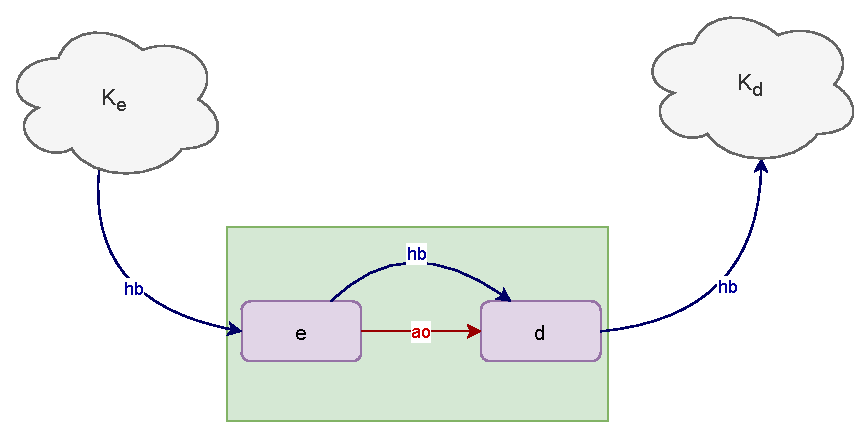
\includegraphics[scale=0.7]{4.InstructionReordering/4.ValidReorderingCandidate/ProofParts/Part1/part1(a).pdf}
        \caption{For any Candidate Execution of $C$, the set $K_e$ and $K_d$ and its relation with events $e,d$.}
        \label{reord:preserve_hb(a)}
    \end{figure}
    
    Consider two events $\event{p1}{K_e}$ and $\event{p2}{K_d}$ (When $e$ is the first event or $d$ is the last event, assume dummy events that can act as $p1$ or $p2$.) belonging to the same agent as that of $e$ and $d$ such that in $C$:
    \begin{align*}
        dir(p1,e)\ \wedge\ dir(d,p2).
    \end{align*}
    
    Note that in terms of direct happens-before relations, on reordering, any $Candidate Execution$ of $C$ will have the following changes shown in Figure~\ref{reord:preserve_hb(b)}
    \begin{figure}[H]
        \centering
        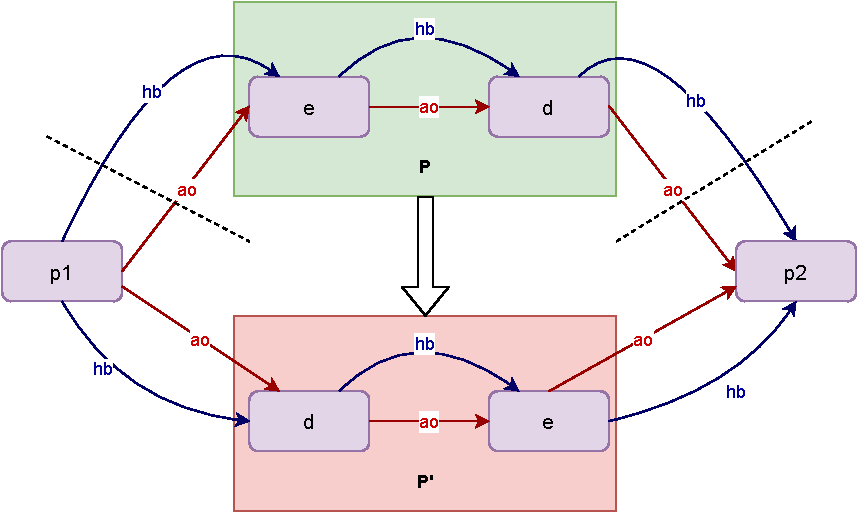
\includegraphics[scale=0.7]{4.InstructionReordering/4.ValidReorderingCandidate/ProofParts/Part1/part1(b).pdf}
        \caption{The \textit{direct happens-before} relation that change while reordering events $e$ and $d$.}
        \label{reord:preserve_hb(b)}
    \end{figure}
    
    The figure above is to show that, for any $Candidate Execution$ of $C$, the following is true
    \[
        cons(p1,e) \ \wedge dir(p1,e) \ \wedge dir(e,d) \ \wedge cons(d,p2) \ \wedge \ dir(d,p2).
    \]
    and for that of $C'$,
    \[
        cons(p1,d) \ \wedge \ dir(p1,d) \ \wedge \ dir(d,e) \ \wedge cons(e,p2) \ \wedge dir(e,p2).
    \]
    
    We need the following key relations to be preserved in Candidate executions of $C'$ 
    \begin{tasks}(2)
        \task $\reln{p1}{hb}{e}.$
        \task $\reln{e}{hb}{k}.$
        \task $\reln{d}{hb}{p2}.$
        \task $\reln{k}{hb}{d}.$ 
    \end{tasks}

    After reordering, we have (a) and (c) preserved due to transitivity  
    \begin{gather*}
        \reln{p1}{hb}{d} \ \wedge \ \reln{d}{hb}{e} \ \Rightarrow \ \reln{p1}{hb}{e}. \\
        \reln{e}{hb}{p2} \ \wedge \ \reln{d}{hb}{e} \ \Rightarrow \ \reln{d}{hb}{p2}. \\
        \reln{p1}{hb}{d} \ \wedge \ \reln{d}{hb}{e} \ \wedge \ \reln{e}{hb}{p2} \ \Rightarrow \ \reln{p1}{hb}{p2}. 
    \end{gather*}

    (b) and (d) may not be preserved due to $\reln{d}{sw}{k}$ or $\reln{k}{sw}{d}$. If we can "pivot" the  set $K_e$ to $p1$ and $K_d$ to $p2$, it would ensure that our other two intended relations also remain preserved after reordering by transitivity. To state formally, we have a valid pair of pivots $<p1,p2>$ when the following two conditions hold
    \begin{gather*}
        \forall \ k \in K_e - \{p1\}, \ \reln{k}{hb}{p1}. \\
        \forall \ k \in K_d - \{p2\}, \ \reln{p2}{hb}{k}.
    \end{gather*}
    
    By Lemma \ref{Lemma1} and \ref{Lemma2} respectively, we have for $C$, the following condition where $<p1, p2>$ is a valid pivot pair.
    \begin{gather*}
        \et{e}{uo} \vee (\et{e}{sc} \wedge \event{e}{W}). \\
        \et{d}{uo} \vee (\et{d}{sc} \wedge \event{d}{R}).
    \end{gather*}
        
    Figure~\ref{reord:preserve_hb_table} summarizes the cases where we have a valid pair of pivots\footnotemark $<p1,p2>$.
    \begin{figure}[H]
        \centering
        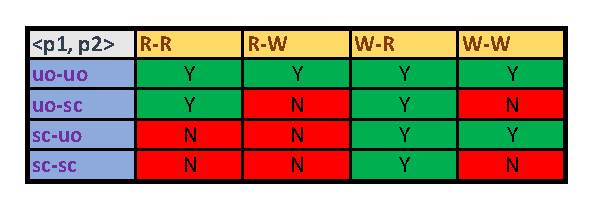
\includegraphics[scale=0.7]{4.InstructionReordering/4.ValidReorderingCandidate/ProofParts/Part1/part1_table.pdf}
        \caption{Table summarizing whether we have valid pair of pivots based on  $e$ and $d$.}
        \label{reord:preserve_hb_table}
    \end{figure}
            
    We show a simple example (Figure~\ref{reord:preserve_hb(c)} and \ref{reord:preserve_hb(d)}) where we do not have a valid pair of pivots, particularly because $p1$ is not a valid pivot. 
    Note that in this example, $K_e = K_{e1} + K_{e2} + p1 + p_x$
    \begin{figure}[H]
        \centering
        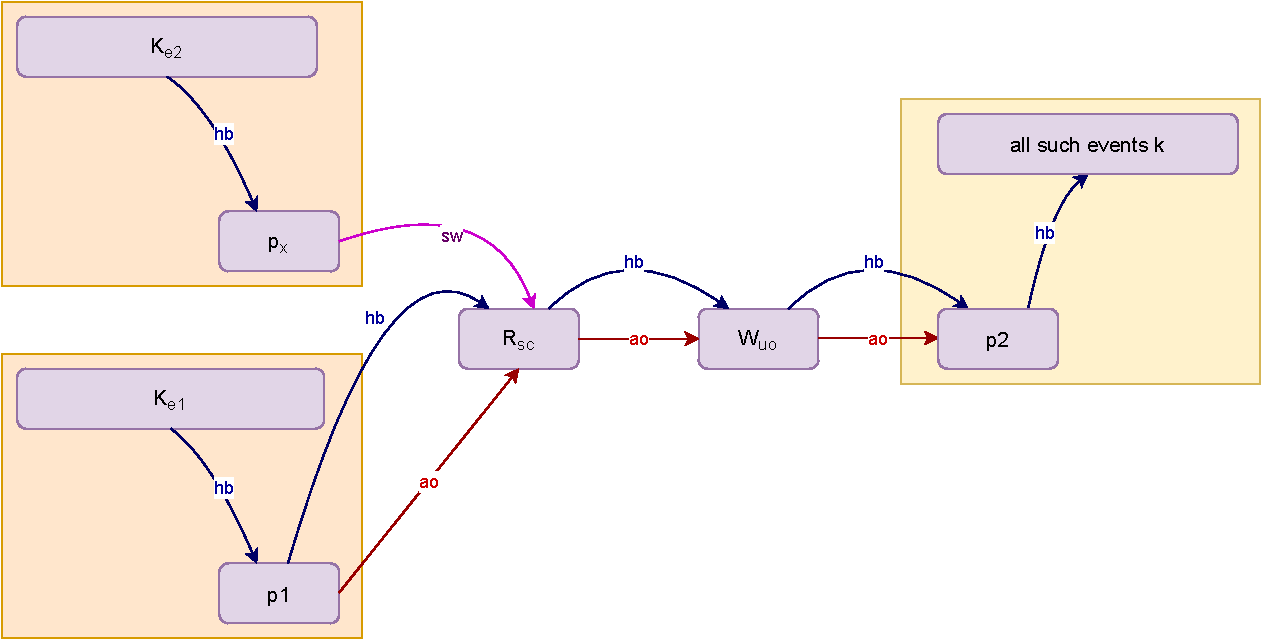
\includegraphics[scale=0.6]{4.InstructionReordering/4.ValidReorderingCandidate/ProofParts/Part1/part1(e).pdf}
        \caption{A Candidate Execution where p1 is not a valid pivot.}
        \label{reord:preserve_hb(c)}
    \end{figure}
    
    %Show figure here of program P'
    \begin{figure}[H]
        \centering
        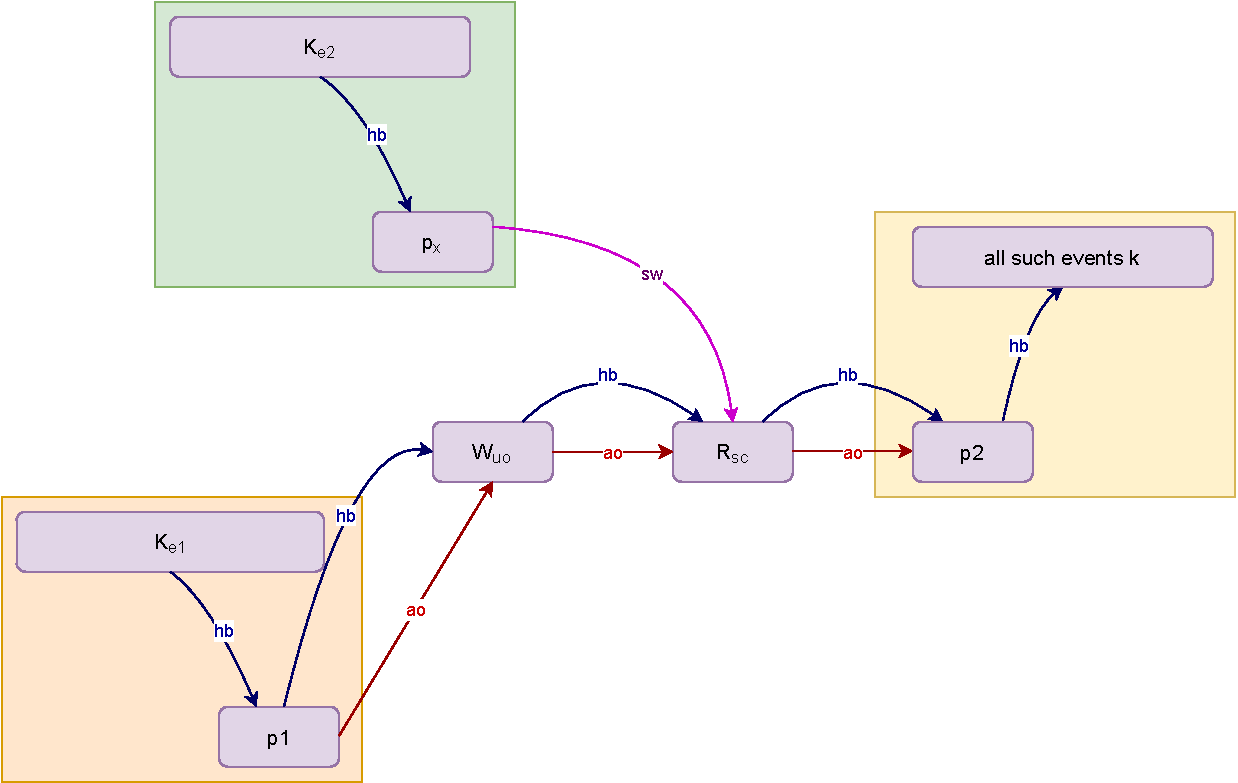
\includegraphics[scale=0.6]{4.InstructionReordering/4.ValidReorderingCandidate/ProofParts/Part1/part1(f).pdf}
        \caption{The resultant Candidate Execution after reordering, exposing the relations with $p_x$, $K_{e2}$ and $d$ that are lost}
        \label{reord:preserve_hb(d)}
    \end{figure}
        
    \footnotetext{This proof does not go about showing the exact happens-before relations that are preserved; rather it uses the properties between different happens before relations that hold, which would imply that for any possible Candidate Execution after reordering, the set of happens-before relations apart from that between $e$ and $d$ remain the same.}
    
\paragraph{2. Additional \textit{happens-before} relations}
    Although we have identified the cases when \textit{happens-before} relations are preserved, we also get some additional relations in some of them.

    %Show an example here and explain
    As an example, for the case when $d$ is a sequentially consistent read, by Lemma \ref{Lemma1}, in any execution of $C$
    \[
        \reln{k}{hb}{d} \centernot\Rightarrow \reln{k}{hb}{e}. 
    \]

    But in $Executions$ of candidate $C'$, by transitivity, we have 
    \[
        \reln{k}{hb}{d} \Rightarrow \reln{k}{hb}{e}. 
    \]

    This is because, there are \textit{happens-before} relations that come through \textit{synchronize-with} relations with $d$. 
    Thus, although we are able to preserve relations that existed in any $Candidate Execution$ of $C$, we also in the process, introduce new ones in $Candidate Executions$ of $C'$. 
    Figures~\ref{reord:add_reln(a)} and \ref{reord:add_reln(b)} shows pictorially an example of a Candidate Execution of $C$ for the case above 
    \begin{figure}[H]
        \centering
        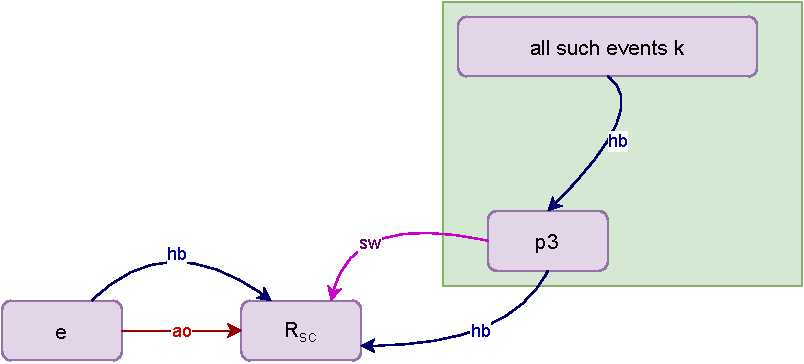
\includegraphics[scale=0.7]{5.InstructionReordering/4.ValidReorderingCandidate/ProofParts/Part2/part2(c).pdf}
        \caption{A Candidate Execution where $d$ read having access mode $sc$.}
        \label{reord:add_reln(a)}
    \end{figure}

    %Show figure here of program P'
    \begin{figure}[H]
        \centering
        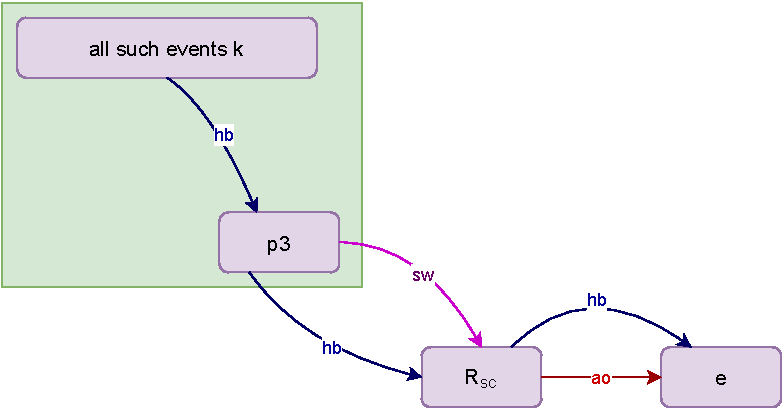
\includegraphics[scale=0.7]{5.InstructionReordering/4.ValidReorderingCandidate/ProofParts/Part2/part2(d).pdf}
        \caption{The Candidate Execution after reordering $e$ and $d$, exposing the new relations established with $e$, $p3$ and set $k$}
        \label{reord:add_reln(b)}
    \end{figure}

    Figure~\ref{reord:add_reln_table} below shows the cases where new relations could be introduced. 
    \begin{figure}[H]
        \centering
        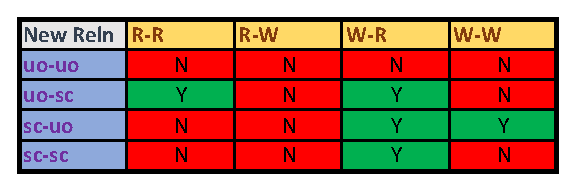
\includegraphics[scale=0.7]{5.InstructionReordering/4.ValidReorderingCandidate/ProofParts/Part2/part2_table.pdf}
        \caption{Table summarizing new \textit{happens-before} relations that could be introduced on having valid pair of pivots.}
        \label{reord:add_reln_table}
    \end{figure}

    For these cases, we investigate whether the new relations introduce new observable behaviors. 

    \paragraph{3. Presence of Cycles?}
        
Because no new $\stck{_{hb}}$ relations are introduced, and because original candidate executions have $\stck{_{hb}}$ as a strict partial order, no cycles are introduced after elimination. 


    \paragraph{4. Do the lost relations result in New Observable Behaviors?}

        To answer this, we need to see whether the relations removed had an impact on $\stck{_{rf}}$ relations other than those with $e$. To prove that it does not have any impact, we divide our argument into two parts, viz. into the two types of relations removed:

        \begin{tasks}(2)
            \task $\reln{k}{hb}{R_uo}$ 
            \task $\reln{R_uo}{hb}{k}$ 
        \end{tasks}

        In the first case, we have the following possibilities. 
        \begin{figure}[H]
            \centering
            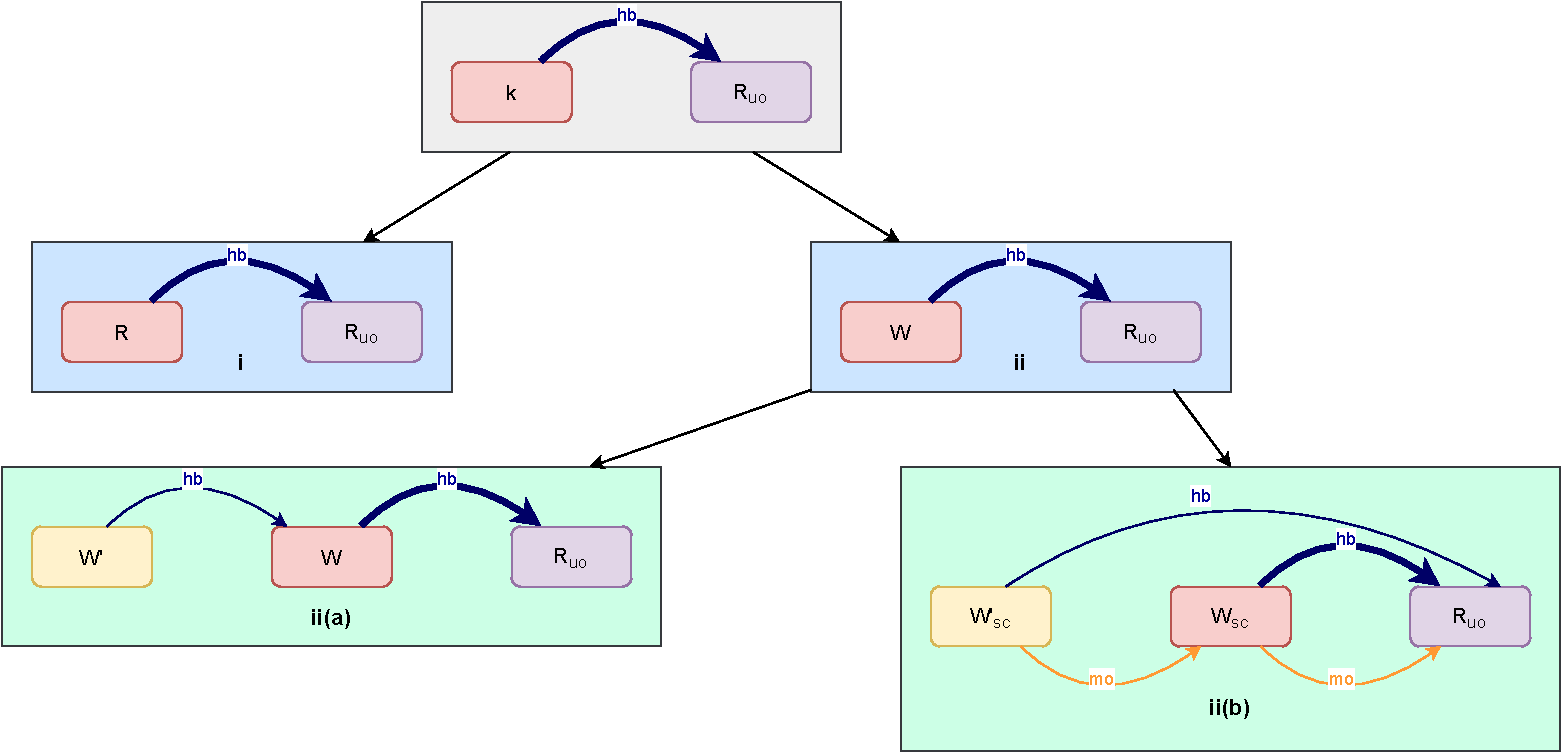
\includegraphics[scale=0.5]{6.Elimination/1.ValidEliminationCandidate/ReadElimProof/ProofParts/Part4_Case1.pdf}
            \caption{The first type of relations removed and the various patterns forbidden by them.}
        \end{figure}

        Observations:
        \begin{itemize}
            \item (i) is not a pattern forbidden by the consistency rules.
            \item (ii)(a) is a pattern of Axiom \ref{CoRe}, however, only restricting $\stck{_{rf}}$ relation with $R$ and $W'$(which here is our Unordered Read)
            \item (ii)(b) is a pattern of Axiom \ref{SeqCsAt}, however, once again, only restricting $\stck{_{rf}}$ relation with $R$ and $W'$. 
        \end{itemize}

        In the second case, we have the following possibilites.
        \begin{figure}[H]
            \centering
            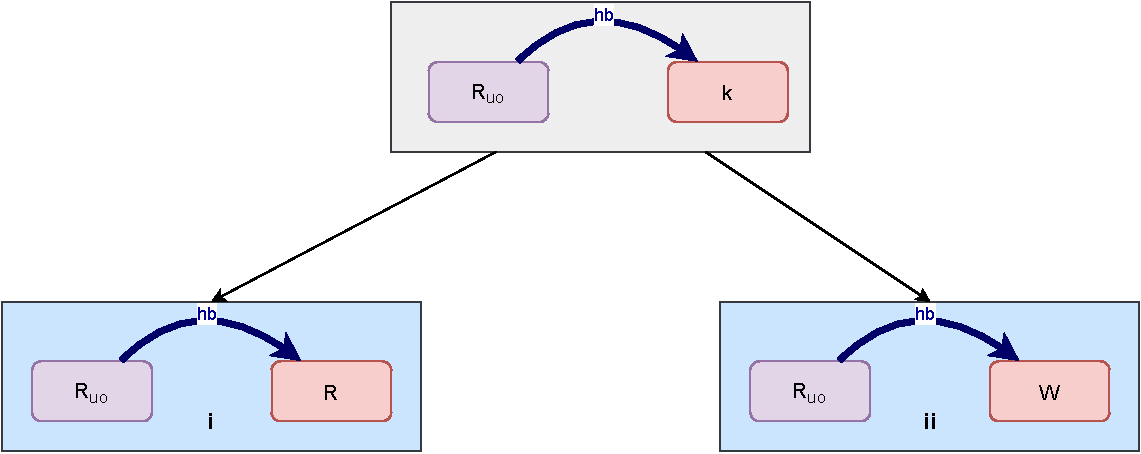
\includegraphics[scale=0.5]{6.Elimination/1.ValidEliminationCandidate/ReadElimProof/ProofParts/Part4_Case2.pdf}
            \caption{The second type of relations removed and the various patterns forbidden by them.}
        \end{figure}

        Observations:
        \begin{itemize}
            \item (i) is not a pattern in any Consistency rules
            \item (ii) is a pattern of Axiom \ref{CoRe}, however, only restricting $\stck{_{rf}}$ relation with $R$ and $W$
        \end{itemize}

        From the above observations, we can infer that the relations removed only have restriction on reads-from relations on the event $e$ we eliminate. Thus, we can conclude that no new observable behaviors are introduced due to the removed $\stck{_{hb}}$ relations. 
    
\end{proof}

    \begin{corollary}
    Consider a Candidate C of a program and its Candidate Executions which are valid. Consider two write events $e$ and $d$ both having equal ranges such that $\neg \cons{e}{d}$ is true in C, $e$ is of type unordered and $\reln{e}{ao}{d}$. 
    Consider another Candidate C' without the event $e$.  
    Then, the set of Observable behaviors possible in C' is a subset of C only if the following holds true.
    \begin{align*}
        \forall \ i \ \in \ [1,n-1] \ \textit{s.t.} \
        \reln{e}{ao}{k_1} \ \wedge \ \reln{k_n}{ao}{d} \ \wedge \ \reln{k_i}{ao}{k_{i+1}} \ \wedge \  
        \cons{e}{k_1} \ \wedge \ \cons{k_n, d} \ \wedge \ \cons{k_i, k_{i+1}}, \\
        \exists \ (n + 1) \geq j > 0 \ \textit{s.t.} \ 
        \forall l \ \in \ [1,j-1] \ . \ Reord(e, k_l) \ 
        \wedge \ 
        \forall m \ \in \ [j,n] \ . \ Reord(k_m, d) 
    \end{align*}
            
    
\end{corollary}

\begin{proof}

    We prove this using induction on the number of events $k$ between $e$ and $d$. For each case, we see whether a valid $j$ exists. 

    \paragraph{Base Case (n=1)}

        For this case, if we have $Reord(e,k1)$ then $j=2$ is a valid choice. By Theorem of reordering, we get Candidate $C''$ with $\cons(e,d)$ whose observable behaviors are a subset. By Theroem (write elim), a observable behaviors of $C'$ is a subset of that of $C''$. By transitivity property of subsets, behaviors of $C'$ is a subset of $C$. 
        
        \critic{blue}{Write above arguments properly}
    
        While if we have $Reord(k1,d)$ then $j=1$ is a valid choice. The argument is the same as above. 
        
    \paragraph{Inductive Case (n)}
        
        Suppose the corollary holds for the case $n$. Meaning, the observable behaviors of $C'$ is a subset of $C$. And suppose $j$ is alos the number as needed. 

        Then for the case where there are $n+1$ events,we have the following two cases:

        If $k_x$ is the additonal event added in between $e$ and $d$, then, if $Reord(k_x, d) \wedge x>j$, the new $j$ remains the same as the old one. Because $Reord(K_{n+1}, d)$, by theorem of reordering, the Candidate $C''$ after reordering has observable behaviors as a subset of $C$. Now after reordering, we have our inductive case assumption, hence observable behaviors of $C'$ is a subset of $C$. 
        
        On the other hand, if $Reord(e,k_x) \wedge x \leq j$, the new $j$ is plus one the old $j$. Because $Reord(e,k_1)$  by theorem of reordering $e$ and $k_1$, the Candidate $C''$ after reordering has observable behaviors as a subset of $C$. Now $j$ for $C''$ becomes $j-1$, hence we get our original inductive case assumption on $n$. By transitive property of subsets observable behaviors of $C'$ is a subset of $C$. 

        \critic{red}{Very rudimentary format of arguments, discuss with Clark and get them more formal}

    
\end{proof}

\begin{proof}
    We prove by induction on the number of events $k$ between $e$ and $d$. We verify that if a $j$ exists that is valid, the Observable behaviors of $C'$ is a subset of $C$.

    \paragraph{Base Case : n = 1}

        We have the case when:
        \begin{align*}
            \reln{e}{ao}{k_1} \ \wedge \ reln{k_1}{ao}{d}
        \end{align*}
        We can divide this into two cases one with $Reord(e, k_1)$ and one with $Reord(k_1, d)$.

        In the first case, note that $j=2$ is the valid choice. Thus, by Theorem of Reordering and Def of consecutive events and agent order, we can reorder $e$ and $k_1$, thus giving us a Candidate $C''$ with :
        \begin{align*}
            \reln{k_1}{ao}{e} \ \wedge \ \reln{e}{ao}{d}
        \end{align*}  
        whose observable behaviors are a subset of $C$

        Due to Def of Consecutive instructions and Theorem of Elmination, we can eliminate $e$, thus giving us 
        \begin{align*}
            \reln{k_1}{ao}{d}
        \end{align*} 

\end{proof}

    %Write elimination
    \subsection{Elimination of Writes}

        The following theorem establishes the condition when we can eliminate a write from a Candidate, given that we have another write consecutive to it.  
            %Write Elimination 
    \begin{theorem} 

    Consider a candidate $C$ of a program and its possible \textit{Candidate Executions} where $\stck{_\textit{hb}}$ is strictly partial order. Consider two events $e$ and $d$ such that $\cons{e}{d}$ is true in $C$ and  $\reln{e}{ao}{d}$. Consider another candidate $C'$ resulting after reordering $e$ and $d$. 
    Then if \emph{Reord(e,d)} is true in $C$, the set observable behaviors possible due to Candidate Executions of $C'$ is a subset of that of $C$. 
\end{theorem}


    \begin{proof}
    We look at this as an elimination of $e$ that takes place in any candidate execution of $C$. 
    We then go about answering the same four questions as we did for reordering. 
    The only major change here being that elimination implies removal $\stck{_{hb}}$ relations, in contrast to introducing new ones.
    We must check whether the removal of these relations introduce new behaviors.
    
    
\paragraph{1. Preserving \textit{happens-before} relations}
        
    If $\stck{_{hb}}$ relations among events are lost after reordering, they may introduce new observable behaviors. The relations that are subject to change can be divided into four parts using events $e$ and $d$.
    \begin{tasks}(2)
        \task $\reln{k}{hb}{e}$.
        \task $\reln{e}{hb}{k}$.
        \task $\reln{d}{hb}{k}$.
        \task $\reln{k}{hb}{d}$.
    \end{tasks}

    Firstly, note that the relations of the form $\reln{e}{hb}{k}$ come through either a $\stck{_{sw}}$ relation with $e$ or relations through event $d$, i.e. of the form $\reln{d}{hb}{k}$. 
    The ones that come due to the latter, may not be preserved after reordering. 
    Note also that, a similar argument exists for relations of the form $\reln{k}{hb}{d}$ wherein relations derived through $e$($\reln{k}{hb}{e}$) may be lost after reordering. 

    Hence, the relations that could be subject to change can be addressed by considering two disjoint sets of events in any \textit{Candidate Execution} of $C$ as below.
    \begin{align*}
       K_e = \{k \ | \ \reln{k}{hb}{e} \}. \\
       K_d = \{k \ | \ \reln{d}{hb}{k} \}. 
    \end{align*}

    Figure~\ref{reord:preserve_hb(a)} below pictorially shows this.
    \begin{figure}[H]
        \centering
        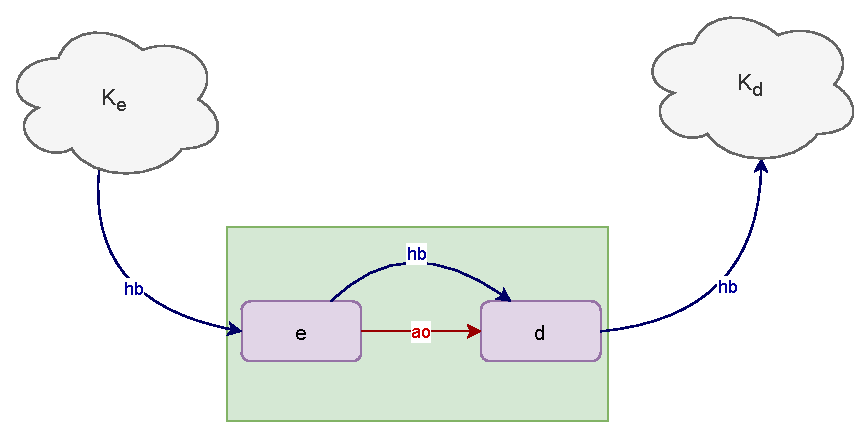
\includegraphics[scale=0.7]{4.InstructionReordering/4.ValidReorderingCandidate/ProofParts/Part1/part1(a).pdf}
        \caption{For any Candidate Execution of $C$, the set $K_e$ and $K_d$ and its relation with events $e,d$.}
        \label{reord:preserve_hb(a)}
    \end{figure}
    
    Consider two events $\event{p1}{K_e}$ and $\event{p2}{K_d}$ (When $e$ is the first event or $d$ is the last event, assume dummy events that can act as $p1$ or $p2$.) belonging to the same agent as that of $e$ and $d$ such that in $C$:
    \begin{align*}
        dir(p1,e)\ \wedge\ dir(d,p2).
    \end{align*}
    
    Note that in terms of direct happens-before relations, on reordering, any $Candidate Execution$ of $C$ will have the following changes shown in Figure~\ref{reord:preserve_hb(b)}
    \begin{figure}[H]
        \centering
        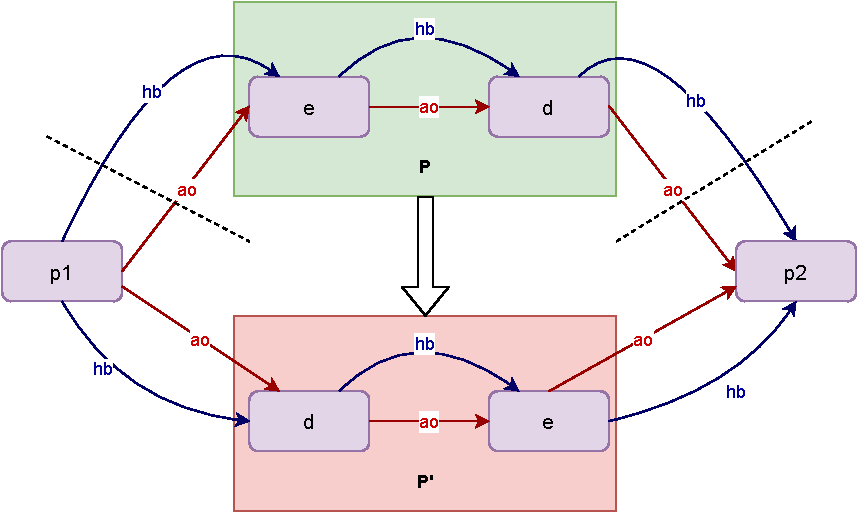
\includegraphics[scale=0.7]{4.InstructionReordering/4.ValidReorderingCandidate/ProofParts/Part1/part1(b).pdf}
        \caption{The \textit{direct happens-before} relation that change while reordering events $e$ and $d$.}
        \label{reord:preserve_hb(b)}
    \end{figure}
    
    The figure above is to show that, for any $Candidate Execution$ of $C$, the following is true
    \[
        cons(p1,e) \ \wedge dir(p1,e) \ \wedge dir(e,d) \ \wedge cons(d,p2) \ \wedge \ dir(d,p2).
    \]
    and for that of $C'$,
    \[
        cons(p1,d) \ \wedge \ dir(p1,d) \ \wedge \ dir(d,e) \ \wedge cons(e,p2) \ \wedge dir(e,p2).
    \]
    
    We need the following key relations to be preserved in Candidate executions of $C'$ 
    \begin{tasks}(2)
        \task $\reln{p1}{hb}{e}.$
        \task $\reln{e}{hb}{k}.$
        \task $\reln{d}{hb}{p2}.$
        \task $\reln{k}{hb}{d}.$ 
    \end{tasks}

    After reordering, we have (a) and (c) preserved due to transitivity  
    \begin{gather*}
        \reln{p1}{hb}{d} \ \wedge \ \reln{d}{hb}{e} \ \Rightarrow \ \reln{p1}{hb}{e}. \\
        \reln{e}{hb}{p2} \ \wedge \ \reln{d}{hb}{e} \ \Rightarrow \ \reln{d}{hb}{p2}. \\
        \reln{p1}{hb}{d} \ \wedge \ \reln{d}{hb}{e} \ \wedge \ \reln{e}{hb}{p2} \ \Rightarrow \ \reln{p1}{hb}{p2}. 
    \end{gather*}

    (b) and (d) may not be preserved due to $\reln{d}{sw}{k}$ or $\reln{k}{sw}{d}$. If we can "pivot" the  set $K_e$ to $p1$ and $K_d$ to $p2$, it would ensure that our other two intended relations also remain preserved after reordering by transitivity. To state formally, we have a valid pair of pivots $<p1,p2>$ when the following two conditions hold
    \begin{gather*}
        \forall \ k \in K_e - \{p1\}, \ \reln{k}{hb}{p1}. \\
        \forall \ k \in K_d - \{p2\}, \ \reln{p2}{hb}{k}.
    \end{gather*}
    
    By Lemma \ref{Lemma1} and \ref{Lemma2} respectively, we have for $C$, the following condition where $<p1, p2>$ is a valid pivot pair.
    \begin{gather*}
        \et{e}{uo} \vee (\et{e}{sc} \wedge \event{e}{W}). \\
        \et{d}{uo} \vee (\et{d}{sc} \wedge \event{d}{R}).
    \end{gather*}
        
    Figure~\ref{reord:preserve_hb_table} summarizes the cases where we have a valid pair of pivots\footnotemark $<p1,p2>$.
    \begin{figure}[H]
        \centering
        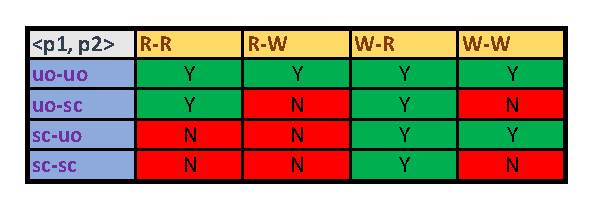
\includegraphics[scale=0.7]{4.InstructionReordering/4.ValidReorderingCandidate/ProofParts/Part1/part1_table.pdf}
        \caption{Table summarizing whether we have valid pair of pivots based on  $e$ and $d$.}
        \label{reord:preserve_hb_table}
    \end{figure}
            
    We show a simple example (Figure~\ref{reord:preserve_hb(c)} and \ref{reord:preserve_hb(d)}) where we do not have a valid pair of pivots, particularly because $p1$ is not a valid pivot. 
    Note that in this example, $K_e = K_{e1} + K_{e2} + p1 + p_x$
    \begin{figure}[H]
        \centering
        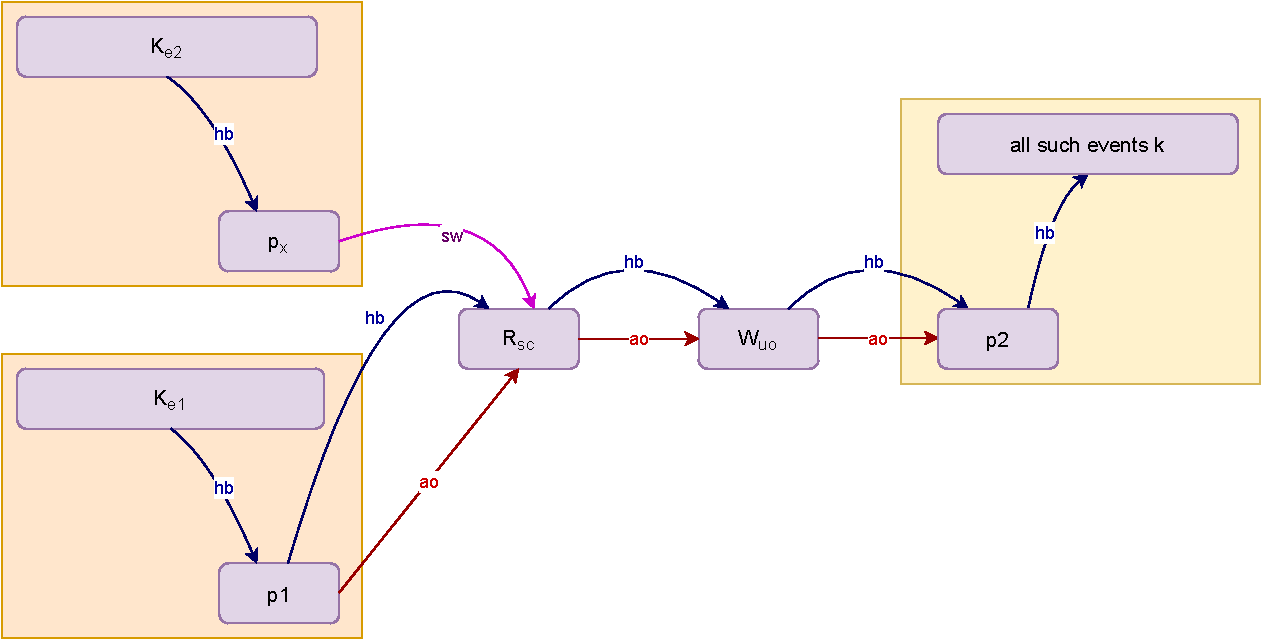
\includegraphics[scale=0.6]{4.InstructionReordering/4.ValidReorderingCandidate/ProofParts/Part1/part1(e).pdf}
        \caption{A Candidate Execution where p1 is not a valid pivot.}
        \label{reord:preserve_hb(c)}
    \end{figure}
    
    %Show figure here of program P'
    \begin{figure}[H]
        \centering
        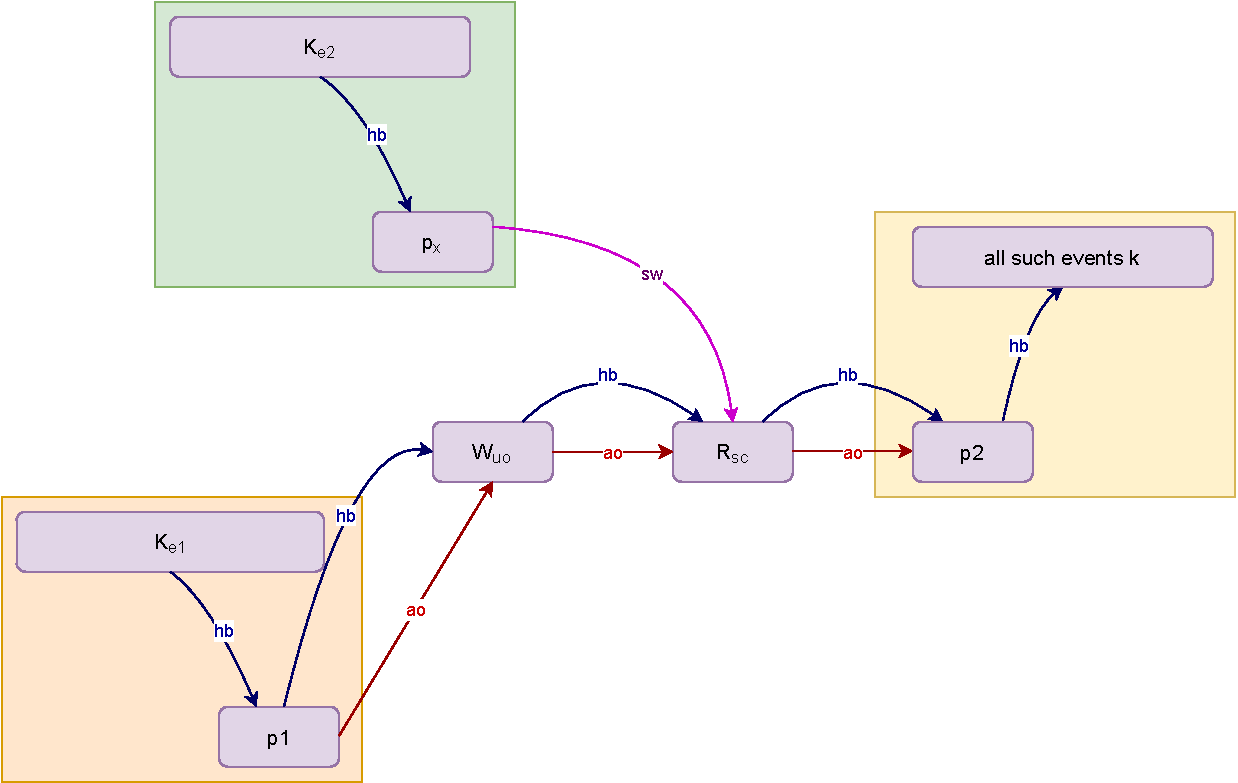
\includegraphics[scale=0.6]{4.InstructionReordering/4.ValidReorderingCandidate/ProofParts/Part1/part1(f).pdf}
        \caption{The resultant Candidate Execution after reordering, exposing the relations with $p_x$, $K_{e2}$ and $d$ that are lost}
        \label{reord:preserve_hb(d)}
    \end{figure}
        
    \footnotetext{This proof does not go about showing the exact happens-before relations that are preserved; rather it uses the properties between different happens before relations that hold, which would imply that for any possible Candidate Execution after reordering, the set of happens-before relations apart from that between $e$ and $d$ remain the same.}
    
\paragraph{2. Additional \textit{happens-before} relations}
    Although we have identified the cases when \textit{happens-before} relations are preserved, we also get some additional relations in some of them.

    %Show an example here and explain
    As an example, for the case when $d$ is a sequentially consistent read, by Lemma \ref{Lemma1}, in any execution of $C$
    \[
        \reln{k}{hb}{d} \centernot\Rightarrow \reln{k}{hb}{e}. 
    \]

    But in $Executions$ of candidate $C'$, by transitivity, we have 
    \[
        \reln{k}{hb}{d} \Rightarrow \reln{k}{hb}{e}. 
    \]

    This is because, there are \textit{happens-before} relations that come through \textit{synchronize-with} relations with $d$. 
    Thus, although we are able to preserve relations that existed in any $Candidate Execution$ of $C$, we also in the process, introduce new ones in $Candidate Executions$ of $C'$. 
    Figures~\ref{reord:add_reln(a)} and \ref{reord:add_reln(b)} shows pictorially an example of a Candidate Execution of $C$ for the case above 
    \begin{figure}[H]
        \centering
        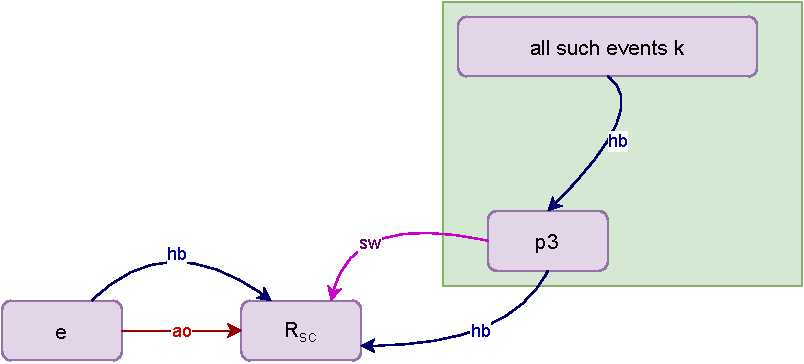
\includegraphics[scale=0.7]{5.InstructionReordering/4.ValidReorderingCandidate/ProofParts/Part2/part2(c).pdf}
        \caption{A Candidate Execution where $d$ read having access mode $sc$.}
        \label{reord:add_reln(a)}
    \end{figure}

    %Show figure here of program P'
    \begin{figure}[H]
        \centering
        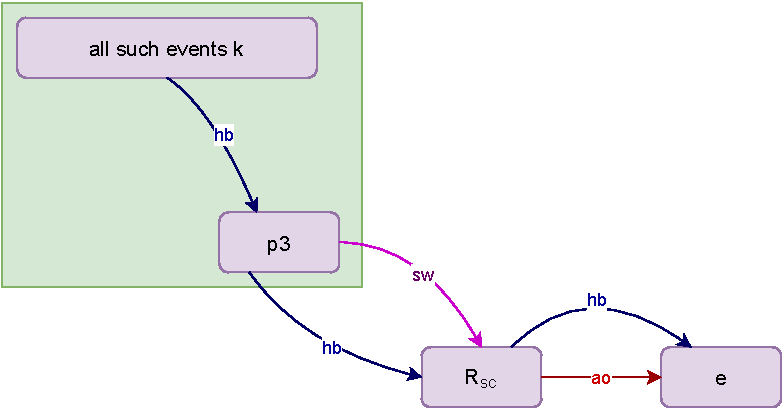
\includegraphics[scale=0.7]{5.InstructionReordering/4.ValidReorderingCandidate/ProofParts/Part2/part2(d).pdf}
        \caption{The Candidate Execution after reordering $e$ and $d$, exposing the new relations established with $e$, $p3$ and set $k$}
        \label{reord:add_reln(b)}
    \end{figure}

    Figure~\ref{reord:add_reln_table} below shows the cases where new relations could be introduced. 
    \begin{figure}[H]
        \centering
        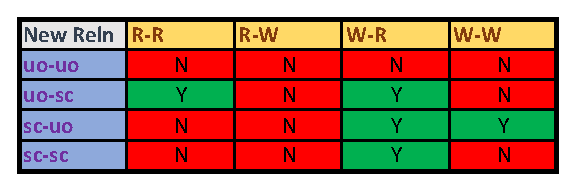
\includegraphics[scale=0.7]{5.InstructionReordering/4.ValidReorderingCandidate/ProofParts/Part2/part2_table.pdf}
        \caption{Table summarizing new \textit{happens-before} relations that could be introduced on having valid pair of pivots.}
        \label{reord:add_reln_table}
    \end{figure}

    For these cases, we investigate whether the new relations introduce new observable behaviors. 

    \paragraph{3. Presence of Cycles?}
        
Because no new $\stck{_{hb}}$ relations are introduced, and because original candidate executions have $\stck{_{hb}}$ as a strict partial order, no cycles are introduced after elimination. 


    \paragraph{4. Do the lost relations result in New Observable Behaviors?}

        To answer this, we need to see whether the relations removed had an impact on $\stck{_{rf}}$ relations other than those with $e$. To prove that it does not have any impact, we divide our argument into two parts, viz. into the two types of relations removed:

        \begin{tasks}(2)
            \task $\reln{k}{hb}{R_uo}$ 
            \task $\reln{R_uo}{hb}{k}$ 
        \end{tasks}

        In the first case, we have the following possibilities. 
        \begin{figure}[H]
            \centering
            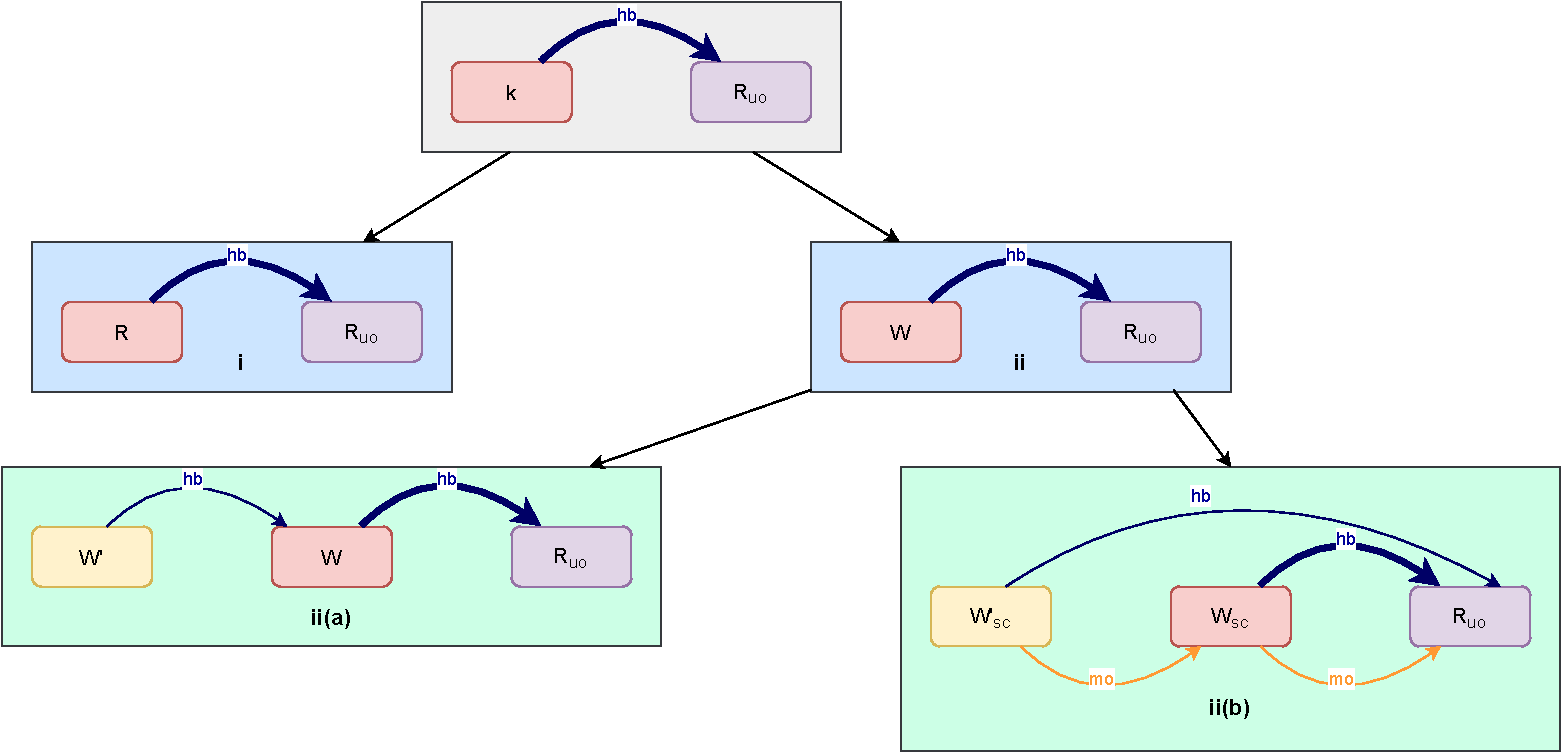
\includegraphics[scale=0.5]{6.Elimination/1.ValidEliminationCandidate/ReadElimProof/ProofParts/Part4_Case1.pdf}
            \caption{The first type of relations removed and the various patterns forbidden by them.}
        \end{figure}

        Observations:
        \begin{itemize}
            \item (i) is not a pattern forbidden by the consistency rules.
            \item (ii)(a) is a pattern of Axiom \ref{CoRe}, however, only restricting $\stck{_{rf}}$ relation with $R$ and $W'$(which here is our Unordered Read)
            \item (ii)(b) is a pattern of Axiom \ref{SeqCsAt}, however, once again, only restricting $\stck{_{rf}}$ relation with $R$ and $W'$. 
        \end{itemize}

        In the second case, we have the following possibilites.
        \begin{figure}[H]
            \centering
            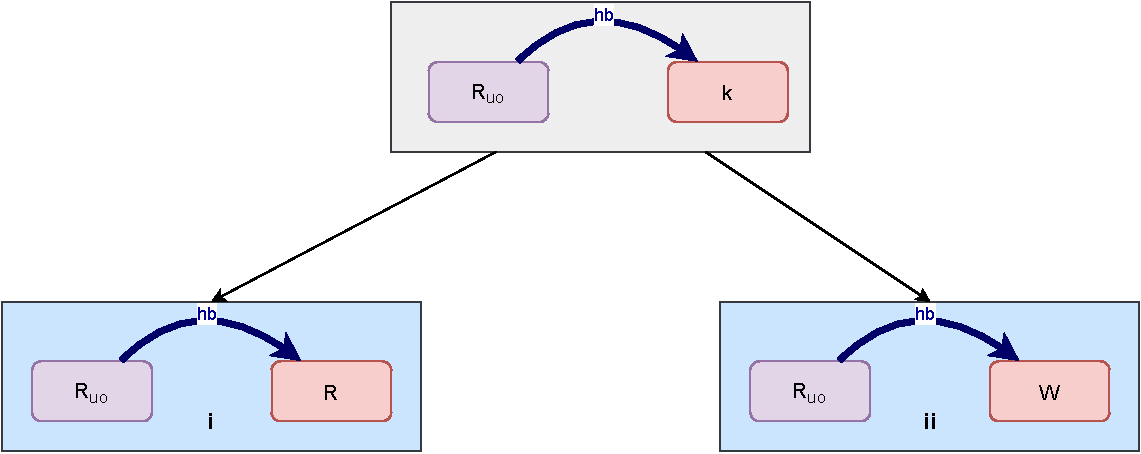
\includegraphics[scale=0.5]{6.Elimination/1.ValidEliminationCandidate/ReadElimProof/ProofParts/Part4_Case2.pdf}
            \caption{The second type of relations removed and the various patterns forbidden by them.}
        \end{figure}

        Observations:
        \begin{itemize}
            \item (i) is not a pattern in any Consistency rules
            \item (ii) is a pattern of Axiom \ref{CoRe}, however, only restricting $\stck{_{rf}}$ relation with $R$ and $W$
        \end{itemize}

        From the above observations, we can infer that the relations removed only have restriction on reads-from relations on the event $e$ we eliminate. Thus, we can conclude that no new observable behaviors are introduced due to the removed $\stck{_{hb}}$ relations. 
    
\end{proof}

    \begin{corollary}
    Consider a Candidate C of a program and its Candidate Executions which are valid. Consider two write events $e$ and $d$ both having equal ranges such that $\neg \cons{e}{d}$ is true in C, $e$ is of type unordered and $\reln{e}{ao}{d}$. 
    Consider another Candidate C' without the event $e$.  
    Then, the set of Observable behaviors possible in C' is a subset of C only if the following holds true.
    \begin{align*}
        \forall \ i \ \in \ [1,n-1] \ \textit{s.t.} \
        \reln{e}{ao}{k_1} \ \wedge \ \reln{k_n}{ao}{d} \ \wedge \ \reln{k_i}{ao}{k_{i+1}} \ \wedge \  
        \cons{e}{k_1} \ \wedge \ \cons{k_n, d} \ \wedge \ \cons{k_i, k_{i+1}}, \\
        \exists \ (n + 1) \geq j > 0 \ \textit{s.t.} \ 
        \forall l \ \in \ [1,j-1] \ . \ Reord(e, k_l) \ 
        \wedge \ 
        \forall m \ \in \ [j,n] \ . \ Reord(k_m, d) 
    \end{align*}
            
    
\end{corollary}

\begin{proof}

    We prove this using induction on the number of events $k$ between $e$ and $d$. For each case, we see whether a valid $j$ exists. 

    \paragraph{Base Case (n=1)}

        For this case, if we have $Reord(e,k1)$ then $j=2$ is a valid choice. By Theorem of reordering, we get Candidate $C''$ with $\cons(e,d)$ whose observable behaviors are a subset. By Theroem (write elim), a observable behaviors of $C'$ is a subset of that of $C''$. By transitivity property of subsets, behaviors of $C'$ is a subset of $C$. 
        
        \critic{blue}{Write above arguments properly}
    
        While if we have $Reord(k1,d)$ then $j=1$ is a valid choice. The argument is the same as above. 
        
    \paragraph{Inductive Case (n)}
        
        Suppose the corollary holds for the case $n$. Meaning, the observable behaviors of $C'$ is a subset of $C$. And suppose $j$ is alos the number as needed. 

        Then for the case where there are $n+1$ events,we have the following two cases:

        If $k_x$ is the additonal event added in between $e$ and $d$, then, if $Reord(k_x, d) \wedge x>j$, the new $j$ remains the same as the old one. Because $Reord(K_{n+1}, d)$, by theorem of reordering, the Candidate $C''$ after reordering has observable behaviors as a subset of $C$. Now after reordering, we have our inductive case assumption, hence observable behaviors of $C'$ is a subset of $C$. 
        
        On the other hand, if $Reord(e,k_x) \wedge x \leq j$, the new $j$ is plus one the old $j$. Because $Reord(e,k_1)$  by theorem of reordering $e$ and $k_1$, the Candidate $C''$ after reordering has observable behaviors as a subset of $C$. Now $j$ for $C''$ becomes $j-1$, hence we get our original inductive case assumption on $n$. By transitive property of subsets observable behaviors of $C'$ is a subset of $C$. 

        \critic{red}{Very rudimentary format of arguments, discuss with Clark and get them more formal}

    
\end{proof}

\begin{proof}
    We prove by induction on the number of events $k$ between $e$ and $d$. We verify that if a $j$ exists that is valid, the Observable behaviors of $C'$ is a subset of $C$.

    \paragraph{Base Case : n = 1}

        We have the case when:
        \begin{align*}
            \reln{e}{ao}{k_1} \ \wedge \ reln{k_1}{ao}{d}
        \end{align*}
        We can divide this into two cases one with $Reord(e, k_1)$ and one with $Reord(k_1, d)$.

        In the first case, note that $j=2$ is the valid choice. Thus, by Theorem of Reordering and Def of consecutive events and agent order, we can reorder $e$ and $k_1$, thus giving us a Candidate $C''$ with :
        \begin{align*}
            \reln{k_1}{ao}{e} \ \wedge \ \reln{e}{ao}{d}
        \end{align*}  
        whose observable behaviors are a subset of $C$

        Due to Def of Consecutive instructions and Theorem of Elmination, we can eliminate $e$, thus giving us 
        \begin{align*}
            \reln{k_1}{ao}{d}
        \end{align*} 

\end{proof}
    